\section{合成方法与实验条件比较}
\label{sec:condition-matrix}

本节先概括前人实验得到的规律，再按主要成相过程比较合成方法。表格逐项记录原料与配比、热史、气氛与体系、容器与助熔剂、冷却或生长程序以及产物表征。比较的目的不是拼出推荐配方，而是保留不同研究对象的差异。目标相的直接文献只明确开放体系高温溶液法和单晶X射线结构鉴定；投料、温程、坩埚、助熔剂和冷却程序均未见明确记载，因此记为\texttt{NA}\cite{ababaikeri2024ba5y12zn}。

\subsection{前人实验结论概览}

已有实验首先表明，组成坐标比单一最高温度更能解释Ba--Y--Si--O的成相差异；Y$_2$O$_3$/SiO$_2$比、MoO$_3$用量和冷却速率会共同影响结构类型和晶体质量\cite{kolitsch2009crystal,wierzbickawieczorek2017high}。其次，单晶结构不能代表批量相纯；无Zn陶瓷研究仍检测到副相\cite{yamane2024microstructure,gulay2024navigation}。最后，局部相图能把复现问题转化为可检验的相区问题，并为下一轮投料提供依据\cite{gulay2024navigation}。下文据此比较各路线的实验条件，不把这些近邻结果直接改写为目标相配方。

\subsection{合成条件的统一比较}

图~\ref{fig:route-matrix}把文献记录分为“合成方法—实验条件—产物表征”三层。外加助熔和自熔/熔体路线记录助熔比例、容器接触、冷却与分离、熔体均化和成核；固相陶瓷路线记录混合、压片、煅烧、复磨和复烧；只有文献明确报道机械活化时才列入机械化学；Czochralski路线另行记录籽晶、提拉、旋转和退火。图中连线表示实验条件与表征结果的对应关系，不表示某一变量必然导致特定相。

\begin{figure*}[t]
  \centering
  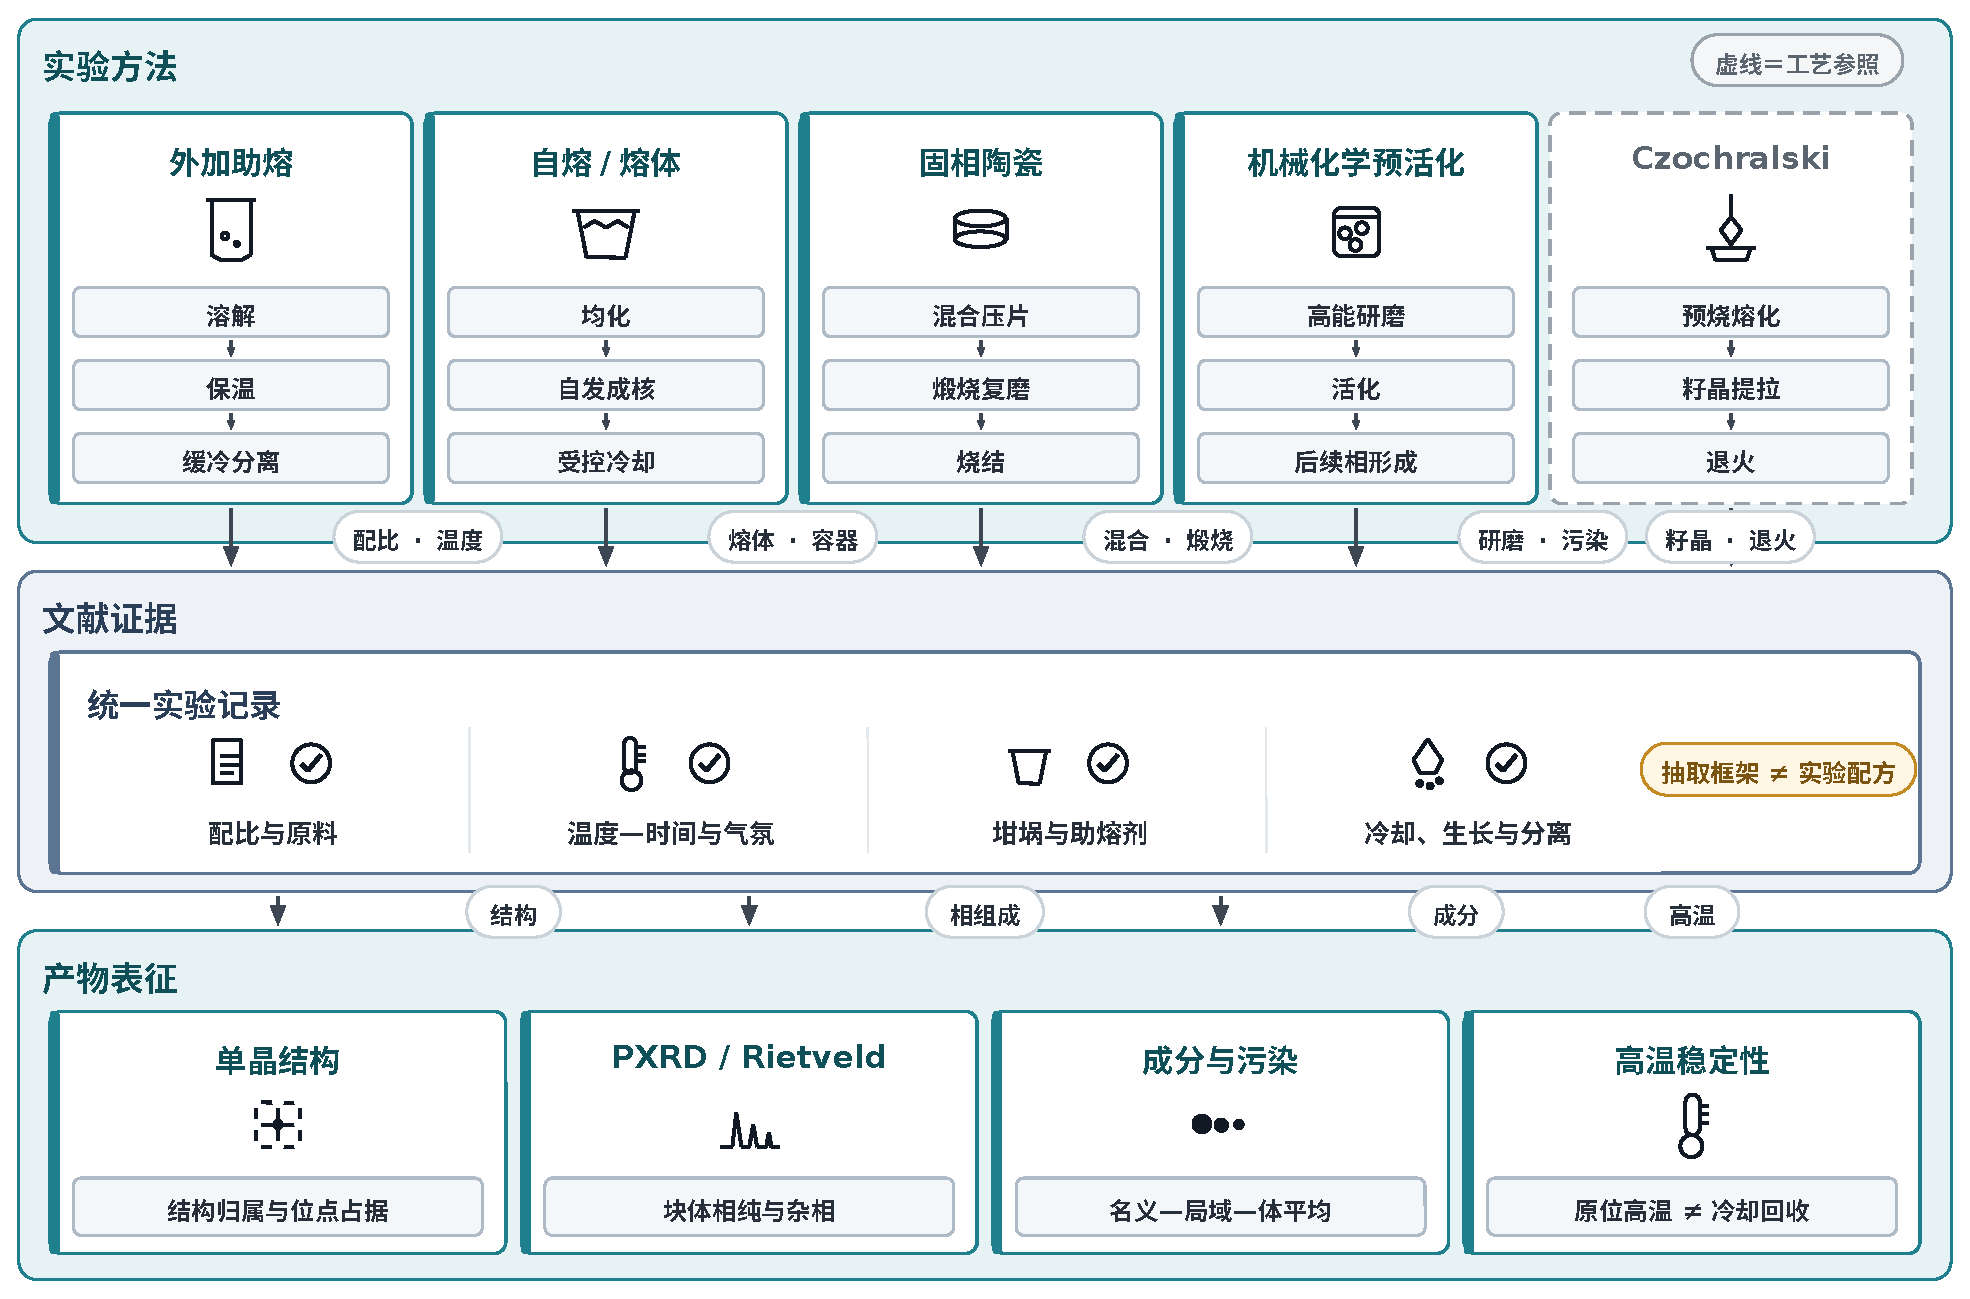
\includegraphics[width=\textwidth]{../figures/pdf/fig02_route_variable_matrix.pdf}
  \caption{不同合成方法的条件比较与产物表征。左侧区分外加助熔、自熔/熔体、固相陶瓷、机械化学预活化与Czochralski；中部列出可比较的原料、热史、气氛、容器、冷却和生长条件；右侧列出单晶结构、PXRD/Rietveld、成分分析及高温稳定性等互补表征。连线表示实验条件与表征结果的对应关系，不表示变量与相形成之间的因果关系；Czochralski仅作工艺参照，本图不是目标相的实验处方。}
  \label{fig:route-matrix}
\end{figure*}

不同方法的文献数量并不代表条件记录同样完整。只有来源明确说明时，才能确认无坩埚熔体、开放体系高温溶液或稀土硅酸盐高温结晶\cite{christensen1994investigation,ababaikeri2024ba3zn4si4o15,leonyuk1999high,giess1982zn2sio4}。Leonyuk的另一条题名级记录只确认单晶对象和结构精修，不能据此判断生长方法\cite{leonyuk1999crystal}。固相记录涵盖结构相变、陶瓷烧结、掺杂表征和玻璃晶化，但只有能定位到实验段的项目才列入数值表格\cite{lin1999phase,zou2021crystal,kerstan2012thermal,cai2024optimized,zhao2026crystal,tejas2024structural,pires2001luminescence,kerstan2015kristallphasen}。机械化学资料中，Tzvetkov与Minkova明确报道机械处理；Yıldırım只报道助剂参与的固--液相烧结，不能因对象是粉体就称为机械化学\cite{tzvetkov2001effects,yldrm2009y2sio5}。提拉法资料同样只作Y$_2$SiO$_5$/Ln$_2$SiO$_5$的工艺参照\cite{pang2005study,alizadeh2021spectroscopy,shoudu1999czochralski,brandle1986czochralski}。

\subsection{条件总表}

表~\ref{tab:synthesis-conditions}采用两块联表。上块记录文献出处、化学输入、合成方法和与目标相的关系；下块以相同编号承接热史、体系、容器与助熔、冷却或生长、产物表征及资料缺失。来源定位写“实验部分”，表示本文核对过原始实验段；写“摘要/题名”，只确认其中明示的对象或方法，不能由“晶体生长”等泛称补出未写明的步骤。\texttt{NA}表示本次核查未取得该项目的明确记载，不表示原实验没有该步骤。

\begin{table*}[!b]
\centering
\footnotesize
\setlength{\tabcolsep}{1.5pt}
\caption{目标化合物及相关体系的合成条件总表（A区：目标化合物直接文献）。目标相与相关体系的数值分区；相关体系数值不是Ba$_5$Y$_{12}$Zn[O(SiO$_4$)]$_8$的已验证配方，不得据此补写缺失条件。}
\label{tab:synthesis-conditions}
\begin{tabular}{P{0.045\textwidth}P{0.19\textwidth}P{0.16\textwidth}P{0.27\textwidth}P{0.13\textwidth}P{0.10\textwidth}}
\toprule
编号 & 来源与定位 & 目标/产物式 & 原料、配比与前处理 & 合成方法 & 与目标相的关系\\
\midrule
A1 & \texttt{ababaikeri2024ba5y12zn}；出版社摘要，ESI仅作结构/成分核验\cite{ababaikeri2024ba5y12zn} & \shortstack[l]{Ba$_5$Y$_{12}$Zn\\{}[O(SiO$_4$)]$_8$} & 原料\texttt{NA}；配比\texttt{NA}；前处理\texttt{NA} & 高温溶液；外加助熔/自助熔未明 & 目标化合物直接文献\\
\bottomrule
\end{tabular}

\vspace{4pt}
\begin{tabular}{P{0.045\textwidth}P{0.15\textwidth}P{0.12\textwidth}P{0.17\textwidth}P{0.15\textwidth}P{0.17\textwidth}P{0.14\textwidth}}
\toprule
编号 & 温度--时间 & 气氛/体系 & 坩埚与助熔 & 冷却/生长 & 产物与表征 & 未明确记载的项目\\
\midrule
A1 & 温度、时间均\texttt{NA} & 开放体系；气体组成\texttt{NA} & 坩埚、助熔剂及用量均\texttt{NA} & 冷却、生长及分离均\texttt{NA} & 单晶；SCXRD；产率、尺寸和批量相纯度\texttt{NA} & 原料、配比、前处理、温时、气体、坩埚、助熔、冷却/分离、产率/尺寸、相分数\\
\bottomrule
\end{tabular}
\end{table*}
\begin{table*}[p]
\ContinuedFloat
\centering
\footnotesize
\renewcommand{\arraystretch}{0.80}
\setlength{\tabcolsep}{1.5pt}
\caption{合成条件总表（续；B区：无Zn的同类Ba--Y四方硅酸盐，不是目标相复现）。}
\begin{tabular}{P{0.045\textwidth}P{0.19\textwidth}P{0.16\textwidth}P{0.27\textwidth}P{0.13\textwidth}P{0.10\textwidth}}
\toprule
编号 & 来源与定位 & 目标/产物式 & 原料、配比与前处理 & 合成方法 & 与目标相的关系\\
\midrule
B1 & \texttt{kolitsch2009crystal}；p.~422，实验部分（伴生相批次）\cite{kolitsch2009crystal} & Ba$_{5+x}$Y$_{13}$Si$_8$O$_{41}$（伴生相） & 整批投料：BaCO$_3$/K$_2$CO$_3$/MoO$_3$各1\,g，Y$_2$O$_3$ 0.1614\,g，SiO$_2$ 0.1718\,g；不可换算为伴生相化学计量配比 & 外加助熔 & 同类Ba--Y四方硅酸盐\\
B2 & \texttt{wierzbickawieczorek2017high}；摘要与系统实验说明，单批SI未取得\cite{wierzbickawieczorek2017high} & Ba$_{5+x}$Y$_{13}$Si$_8$O$_{41}$（151次筛选中的一相） & BaO--K$_2$O--Y$_2$O$_3$--SiO$_2$--MoO$_3$研究体系；试剂形态、单批配比、前处理\texttt{NA} & 外加助熔 & 同类Ba--Y四方硅酸盐\\
B3 & \texttt{yamane2024synthesis}；原文工艺摘录（自熔晶体）\cite{yamane2024synthesis} & Ba$_x$Y$_{26}$Si$_{16}$O$_{71+x}$（$x\approx10.2$） & 原料、精确配比、前处理\texttt{NA} & 自熔/熔体 & 同类Ba--Y四方硅酸盐\\
B4 & \texttt{yamane2024synthesis}；摘要证据（$x=9$--11陶瓷系列）\cite{yamane2024synthesis} & Ba$_x$Y$_{26}$Si$_{16}$O$_{71+x}$（系列） & 原料、各组成点配比、前处理\texttt{NA} & 固相陶瓷 & 同类Ba--Y四方硅酸盐\\
B5 & \texttt{yamane2024microstructure}；p.~598，\S2\cite{yamane2024microstructure} & Ba$_x$Y$_{26}$Si$_{16}$O$_{71+x}$（$x=9$--14系列） & BaCO$_3$/Y$_2$O$_3$/SiO$_2$；Ba:Y:Si=$x$:26:16（$x=9.0$--14.0）；原料热预处理；玛瑙罐/球中400\,rpm干磨1\,h，煅烧后再磨1\,h & 固相陶瓷 & 同类Ba--Y四方硅酸盐\\
B6 & \texttt{gulay2024navigation}；主文\S2.1.1、SI \S1.1/\S1.3\cite{gulay2024navigation} & Ba$_5$Y$_{13}$[SiO$_4$]$_8$O$_{8.5}$（phase A） & BaCO$_3$/Y$_2$O$_3$/SiO$_2$；BaCO$_3$:YO$_{1.5}$:SiO$_2=5{:}13{:}8$，终料0.5\,g；干燥/预热、玛瑙研磨、10\,mm压片 & 固相陶瓷/粉体 & 同类Ba--Y四方硅酸盐\\
\bottomrule
\end{tabular}

\vspace{4pt}
\begin{tabular}{P{0.045\textwidth}P{0.15\textwidth}P{0.12\textwidth}P{0.17\textwidth}P{0.15\textwidth}P{0.17\textwidth}P{0.14\textwidth}}
\toprule
编号 & 温度--时间 & 气氛/体系 & 坩埚与助熔 & 冷却/生长 & 产物与表征 & 未明确记载的项目\\
\midrule
B1 & 1150\,$^\circ$C，3\,h & 空气；开放/封闭性未明；坩埚加盖 & 有盖Pt坩埚；MoO$_3$ 1\,g；蒸馏水溶去助熔相 & 2\,K\,h$^{-1}$冷至900\,$^\circ$C；关炉后慢冷至室温 & 无色棱柱伴生晶体；单晶精修给暂定式；独立产率、批量相分数\texttt{NA} & 伴生相独立化学计量配比/前处理、体系封闭性、独立产率、相分数\\
B2 & 单批温度、时间\texttt{NA}（不把参数扫描范围合并成代表配方） & \texttt{NA} & 坩埚、助熔用量、分离\texttt{NA} & 冷却与生长\texttt{NA} & 多相筛选；SCXRD\slash PXRD\slash Rietveld\slash SEM；该相单批产率\texttt{NA} & 单批配比、前处理、温时、气氛、坩埚、助熔量、冷却、产率\\
B3 & 1600\,$^\circ$C；时间\texttt{NA} & 气氛、开放/封闭\texttt{NA} & 坩埚、助熔组成/用量\texttt{NA} & 冷却与成核\texttt{NA} & 自熔单晶；SCXRD；产率、尺寸、批量相分数\texttt{NA} & 原料、配比、前处理、时间、体系、坩埚、助熔、冷却、产率/尺寸、相分数\\
B4 & 温度、时间\texttt{NA} & \texttt{NA} & 坩埚、外加助熔\texttt{NA} & \texttt{NA} & 陶瓷组成窗口；SCXRD/PXRD的具体分工与相分数\texttt{NA} & 原料、单点配比、前处理、全部热史/体系/容器/冷却、相分数\\
B5 & 1300\,$^\circ$C，12\,h煅烧；1600\,$^\circ$C，2\,h烧成 & 空气；体系封闭性\texttt{NA} & Pt--Rh板；有盖氧化铝坩埚；未列外加助熔 & 断电后炉冷至室温 & 陶瓷；PXRD；见副相及玛瑙来源SiO$_2$污染；定量相分数\texttt{NA} & 升降温速率、体系封闭性、产率/相分数\\
B6 & 1273\,K，12\,h煅烧；1573\,K，24\,h退火并复磨复烧两次；中子样另在1573\,K均化12\,h & 空气；升降温5\,K\,min$^{-1}$ & 氧化铝坩埚；未列助熔剂 & 冷却后破碎细磨；非晶体生长 & 粉体；PXRD监测；EDS、CRED、同步辐射PXRD、中子TOF；产率/定量相分数\texttt{NA} & 独立产率、定量相分数\\
\bottomrule
\end{tabular}
\end{table*}
\begin{table*}[p]
\ContinuedFloat
\centering
\footnotesize
\setlength{\tabcolsep}{1.5pt}
\caption{合成条件总表（续；C区：结构相关和工艺参照的高温溶液与熔体研究）。}
\begin{tabular}{P{0.045\textwidth}P{0.19\textwidth}P{0.16\textwidth}P{0.27\textwidth}P{0.13\textwidth}P{0.10\textwidth}}
\toprule
编号 & 来源与定位 & 目标/产物式 & 原料、配比与前处理 & 合成方法 & 与目标相的关系\\
\midrule
C1 & \texttt{ababaikeri2024ba3zn4si4o15}；出版社摘要\cite{ababaikeri2024ba3zn4si4o15} & Ba$_3$Zn$_4$Si$_4$O$_{15}$ & 原料、配比、前处理\texttt{NA} & 高温溶液；外加/自助熔未明 & 结构相关化合物\\
C2 & \texttt{redhammer2003beta}；IUCr原文实验部分\cite{redhammer2003beta} & $\beta$-Y$_2$Si$_2$O$_7$，伴Na$_2$Si$_2$O$_5$与氧磷灰石 & Na$_2$CO$_3$/Y$_2$O$_3$/SiO$_2$按NaYSi$_2$O$_6$配比；营养物:Na$_2$MoO$_4=1{:}10$；前处理\texttt{NA} & 外加助熔 & 工艺参照研究\\
C3 & \texttt{giess1982zn2sio4}；原始论文记录\cite{giess1982zn2sio4} & Zn$_2$SiO$_4$ & 熔体$5\,$Zn$_2$SiO$_4+3\,$Pb$_2$ZnSi$_2$O$_7$；氟化物供Zn的试验；前处理\texttt{NA} & 外加助熔 & 工艺参照研究\\
C4 & \texttt{christensen1994investigation}；题名/元数据\cite{christensen1994investigation} & 高温稀土焦硅酸盐 & 原料、配比、前处理\texttt{NA} & 无坩埚熔体 & 工艺参照研究\\
C5 & \texttt{leonyuk1999high}；原文索引实验段（助熔支线）\cite{leonyuk1999high} & \shortstack[l]{Y$_2$SiO$_5$/\\Y$_2$Si$_2$O$_7$/\\LaBSiO$_5$} & Y--Si--O营养物；Li/K二、三钼酸盐；精确配比、前处理\texttt{NA} & 外加助熔 & 工艺参照研究\\
C6 & \texttt{leonyuk1999crystal}；题名与DOI元数据\cite{leonyuk1999crystal} & \shortstack[l]{Y$_2$SiO$_5$/\\Y$_2$Si$_2$O$_7$/\\LaBSiO$_5$} & 原料、配比、前处理\texttt{NA} & 未明（题名未区分生长路线） & 工艺参照研究\\
\bottomrule
\end{tabular}

\vspace{4pt}
\begin{tabular}{P{0.045\textwidth}P{0.15\textwidth}P{0.12\textwidth}P{0.17\textwidth}P{0.15\textwidth}P{0.17\textwidth}P{0.14\textwidth}}
\toprule
编号 & 温度--时间 & 气氛/体系 & 坩埚与助熔 & 冷却/生长 & 产物与表征 & 未明确记载的项目\\
\midrule
C1 & 温度、时间\texttt{NA} & 开放空气；气流\texttt{NA} & 坩埚、助熔剂及用量\texttt{NA} & 冷却、生长、分离\texttt{NA} & 单晶；SCXRD；产率、尺寸、相分数\texttt{NA} & 原料、配比、前处理、温时、气流、坩埚/助熔、冷却/分离、产率/尺寸/相分数\\
C2 & 缓升至1473\,K（1200\,$^\circ$C），24\,h & 气氛、开放/封闭\texttt{NA}；坩埚加盖 & 有盖Pt坩埚；Na$_2$MoO$_4$；沸水溶去助熔剂 & 2\,K\,h$^{-1}$冷至673\,K（400\,$^\circ$C）；后续冷却\texttt{NA} & 无色立方晶体及伴生相；100/280\,K SCXRD；产率\texttt{NA} & 前处理、气氛/体系、后续冷却、产率\\
C3 & 1300\,$^\circ$C至960\,$^\circ$C；保温\texttt{NA} & 气氛、开放/封闭\texttt{NA} & 坩埚\texttt{NA}；Pb$_2$ZnSi$_2$O$_7$/氟化物助熔；分离\texttt{NA} & 1\,$^\circ$C\,h$^{-1}$；后续冷却\texttt{NA} & 数毫米六方柱；化学分析/浮力密度，来源式Zn$_{1.96}$Si$_{1.04}$O$_{4.04}$；产率\texttt{NA} & 前处理、保温、体系、坩埚、分离、后续冷却、产率\\
C4 & 温度、时间\texttt{NA} & \texttt{NA} & 无坩埚；助熔\texttt{NA} & \texttt{NA} & 熔体产物；中子粉末衍射/profile refinement；产率、相分数\texttt{NA} & 原料、配比、前处理、温时、体系、助熔、冷却、产率/相分数\\
C5 & 温度、时间\texttt{NA} & \texttt{NA} & Li/K钼酸盐助熔；坩埚、助熔比、分离\texttt{NA} & 冷程\texttt{NA} & 自发成核晶体；电子探针、XRD/结构精修；产率\texttt{NA} & 精确配比、前处理、温时、体系、坩埚、助熔比/分离、冷却、产率\\
C6 & 温度、时间\texttt{NA} & 气氛/体系\texttt{NA} & 坩埚、助熔\texttt{NA} & 生长与冷却参数\texttt{NA} & 题名仅支持单晶对象与结构精修；产率/尺寸\texttt{NA} & 原料、配比、前处理、合成方法及全部实验条件、产率/尺寸\\
\bottomrule
\end{tabular}
\end{table*}
\begin{table*}[p]
\ContinuedFloat
\centering
\footnotesize
\setlength{\tabcolsep}{1.5pt}
\caption{合成条件总表（续；C区：结构相关和工艺参照的固相陶瓷研究，第一组）。}
\begin{tabular}{P{0.045\textwidth}P{0.19\textwidth}P{0.20\textwidth}P{0.23\textwidth}P{0.13\textwidth}P{0.10\textwidth}}
\toprule
编号 & 来源与定位 & 目标/产物式 & 原料、配比与前处理 & 合成方法 & 与目标相的关系\\
\midrule
C7 & \texttt{lin1999phase}；原文实验部分\cite{lin1999phase} & BaZn$_2$Si$_2$O$_7$ & BaCO$_3$/ZnO/SiO$_2$化学计量配比；充分混合并中间研磨 & 固相陶瓷 & 结构相关化合物\\
C8 & \texttt{zou2021crystal}；原始论文PDF实验部分\cite{zou2021crystal} & BaZnSi$_3$O$_8$ & BaCO$_3$（99.8\%）、ZnO/SiO$_2$（99.5\%）；配比\texttt{NA}；聚乙烯罐/ZrO$_2$球/去离子水球磨5\,h，85\,$^\circ$C干燥，150\,MPa压片 & 固相陶瓷 & 结构相关化合物\\
C9 & \texttt{kerstan2012thermal}；原始论文实验部分，批次映射未暴露\cite{kerstan2012thermal} & \shortstack[l]{Ba$_2$ZnSi$_2$O$_7$/\\BaZnSiO$_4$；\\BaZn$_{2-x}$Mg$_x$Si$_2$O$_7$系列} & SiO$_2$/BaCO$_3$/ZnO；Mg源为碳酸盐--氢氧化物水合物；球磨；单批配比/球磨参数\texttt{NA} & 固相陶瓷 & 工艺参照研究\\
C10 & \texttt{cai2024optimized}；题名/元数据\cite{cai2024optimized} & BaZnSi$_3$O$_8$基陶瓷 & 原料、配比、前处理\texttt{NA} & 固相陶瓷 & 工艺参照研究\\
C11 & \texttt{zhao2026crystal}；题名/元数据\cite{zhao2026crystal} & Ba$_2$MgSi$_2$O$_7$陶瓷 & 原料、配比、前处理\texttt{NA} & 固相陶瓷 & 工艺参照研究\\
\bottomrule
\end{tabular}

\vspace{4pt}
\begin{tabular}{P{0.045\textwidth}P{0.15\textwidth}P{0.12\textwidth}P{0.17\textwidth}P{0.15\textwidth}P{0.17\textwidth}P{0.14\textwidth}}
\toprule
编号 & 温度--时间 & 气氛/体系 & 坩埚与助熔 & 冷却/生长 & 产物与表征 & 未明确记载的项目\\
\midrule
C7 & 1280\,$^\circ$C；时间\texttt{NA} & \texttt{NA} & 坩埚、助熔\texttt{NA} & \texttt{NA} & 白色多晶粉；PXRD、中子衍射、GSAS/Rietveld；产率/相分数\texttt{NA} & 时间、体系、坩埚/助熔、冷却、产率/相分数\\
C8 & 空气中1000\,$^\circ$C，3\,h煅烧（5\,$^\circ$C\,min$^{-1}$）；1090--1120\,$^\circ$C，3\,h烧结 & 空气；开放/封闭\texttt{NA} & 坩埚、助熔\texttt{NA} & 2\,$^\circ$C\,min$^{-1}$冷至1000\,$^\circ$C，随后炉冷 & 陶瓷；实验室/同步辐射XRD与Rietveld；产率/定量相分数\texttt{NA} & 配比、体系封闭性、坩埚/助熔、产率/相分数\\
C9 & 单批温程/时间\texttt{NA}（资料只有跨组成总范围，未写入代表配方） & \texttt{NA} & 坩埚、助熔\texttt{NA} & 冷后再球磨；冷速\texttt{NA} & 多晶；HT-XRD、膨胀仪；单批相分数\texttt{NA} & 单批配比/球磨、温时、体系、坩埚/助熔、冷速、相分数\\
C10 & 温度、时间\texttt{NA} & \texttt{NA} & 坩埚、助熔\texttt{NA} & \texttt{NA} & 陶瓷；结构/微波介电表征，具体相纯方法和相分数\texttt{NA} & 原料、配比、前处理及全部实验条件、相分数\\
C11 & 温度、时间\texttt{NA} & \texttt{NA} & 坩埚、助熔\texttt{NA} & \texttt{NA} & 陶瓷；结构/烧结/微波介电表征，具体相纯方法和相分数\texttt{NA} & 原料、配比、前处理及全部实验条件、相分数\\
\bottomrule
\end{tabular}
\end{table*}
\begin{table*}[p]
\ContinuedFloat
\centering
\footnotesize
\setlength{\tabcolsep}{1.5pt}
\caption{合成条件总表（续；C区：结构相关和工艺参照的固相陶瓷研究，第二组）。}
\begin{tabular}{P{0.045\textwidth}P{0.19\textwidth}P{0.16\textwidth}P{0.27\textwidth}P{0.13\textwidth}P{0.10\textwidth}}
\toprule
编号 & 来源与定位 & 目标/产物式 & 原料、配比与前处理 & 合成方法 & 与目标相的关系\\
\midrule
C12 & \texttt{tejas2024structural}；开放原文实验部分\cite{tejas2024structural} & Ba$_2$ZnSi$_2$O$_7$:Sm$^{3+}$ & BaCO$_3$/ZnO/SiO$_2$（99\%），Sm$_2$O$_3$（99.9\%）；名义掺杂比\texttt{NA}；乙醇中玛瑙研钵研磨1\,h & 固相陶瓷 & 工艺参照研究\\
C13 & \texttt{pires2001luminescence}；原始摘要\cite{pires2001luminescence} & Ba/Zn正硅酸盐:Eu$^{3+}$/Mn$^{2+}$ & 氧化物/碳酸盐，或Ba$_2$SiO$_4$:Eu与Zn$_2$SiO$_4$:Mn前驱体；配比、前处理\texttt{NA} & 固相反应 & 工艺参照研究\\
C14 & \texttt{kerstan2015kristallphasen}；学位论文元数据/工艺索引\cite{kerstan2015kristallphasen} & Ba--Zn--Si晶相/高温玻璃焊料晶化相 & 原料、配比、前处理\texttt{NA} & 固相陶瓷（玻璃晶化语境） & 工艺参照研究\\
C15 & \texttt{yldrm2009y2sio5}；机构论文库摘要\cite{yldrm2009y2sio5} & Y$_2$SiO$_5$粉体 & LiYO$_2$添加剂；配比、前处理\texttt{NA} & 固--液相烧结；非机械化学证据 & 工艺参照研究\\
C16 & \texttt{zou2019anti}；原文索引实验部分\cite{zou2019anti} & Ba$_2$ZnSi$_2$O$_7$ & BaCO$_3$（99.8\%）、ZnO/SiO$_2$（99.5\%）；配比\texttt{NA}；聚乙烯罐/ZrO$_2$球/去离子水球磨5\,h & 固相陶瓷 & 工艺参照研究\\
\bottomrule
\end{tabular}

\vspace{4pt}
\begin{tabular}{P{0.045\textwidth}P{0.15\textwidth}P{0.12\textwidth}P{0.17\textwidth}P{0.15\textwidth}P{0.17\textwidth}P{0.14\textwidth}}
\toprule
编号 & 温度--时间 & 气氛/体系 & 坩埚与助熔 & 冷却/生长 & 产物与表征 & 未明确记载的项目\\
\midrule
C12 & O$_2$中1200\,$^\circ$C，6\,h；升温5\,$^\circ$C\,min$^{-1}$ & O$_2$；开放/封闭\texttt{NA} & 氧化铝坩埚；助熔\texttt{NA} & 自然冷至室温后研磨 & 粉体；XRD/FTIR/SEM--EDS/热与光谱；产率/相分数\texttt{NA} & 掺杂比、体系封闭性、助熔、产率/相分数\\
C13 & 温度、时间\texttt{NA} & \texttt{NA} & 坩埚、助熔\texttt{NA} & \texttt{NA} & 粉体；PXRD/IR/UV--vis/发光；产率/相分数\texttt{NA} & 配比、前处理及全部实验条件、产率/相分数\\
C14 & 退火窗口数值与批次对应\texttt{NA} & \texttt{NA} & 坩埚、助熔\texttt{NA} & \texttt{NA} & 晶化相；HT-XRD/膨胀表征索引；单批相分数\texttt{NA} & 原料、配比、前处理及全部单批实验条件、相分数\\
C15 & 完整温程/时间\texttt{NA} & \texttt{NA} & 坩埚\texttt{NA}；LiYO$_2$添加剂用量\texttt{NA} & \texttt{NA} & 粉体；光学显微、XRD、SEM--EDS；产率/相分数\texttt{NA} & 配比、前处理及全部热史/体系/容器/冷却、产率/相分数\\
C16 & 空气中1100\,$^\circ$C，3\,h煅烧；air/O$_2$/N$_2$中1200\,$^\circ$C或N$_2$--1\,vol\% H$_2$中1125\,$^\circ$C烧结；烧结时间\texttt{NA} & air/O$_2$/N$_2$/N$_2$--1\,vol\% H$_2$；开放/封闭\texttt{NA} & 坩埚、助熔\texttt{NA} & \texttt{NA} & 陶瓷；XRD/XPS/微波介电；还原气氛样见BaSiO$_3$；产率/相分数\texttt{NA} & 配比、烧结时间、体系封闭性、坩埚/助熔、冷却、产率/相分数\\
\bottomrule
\end{tabular}
\end{table*}
\begin{table*}[p]
\ContinuedFloat
\centering
\footnotesize
\setlength{\tabcolsep}{1.5pt}
\renewcommand{\arraystretch}{0.94}
\caption{合成条件总表（续；C区：机械活化与Czochralski工艺参照）。}
\begin{tabular}{P{0.045\textwidth}P{0.19\textwidth}P{0.16\textwidth}P{0.27\textwidth}P{0.13\textwidth}P{0.10\textwidth}}
\toprule
编号 & 来源与定位 & 目标/产物式 & 原料、配比与前处理 & 合成方法 & 与目标相的关系\\
\midrule
C17 & \texttt{tzvetkov2001effects}；p.~126，\S2\cite{tzvetkov2001effects} & \shortstack[l]{Y$_2$SiO$_5$/\\Y$_2$Si$_2$O$_7$/\\钇氧磷灰石混相} & Y$_2$O$_3$/SiO$_2=7{:}9$；另比较水合氧化钇；80\,cm$^3$玛瑙罐、20\,mm/总重40\,g玛瑙球，球粉比7:1；空气中256\,rpm，1--3\,h & 机械化学预活化+后续热处理 & 工艺参照研究\\
C18 & \texttt{pang2005study}；原文实验部分\cite{pang2005study} & Y$_2$SiO$_5$ & Y$_2$O$_3$（99.999\%）/SiO$_2$（99.99\%），约980\,g、化学计量配比；刚玉研钵混磨、液压压块并预烧 & Czochralski & 工艺参照研究\\
C19 & \texttt{leonyuk1999high}；原文索引实验段（提拉支线）\cite{leonyuk1999high} & Y$_2$SiO$_5$（含Cr掺杂系列） & 高纯Y$_2$O$_3$/SiO$_2$；精确配比、预烧\texttt{NA} & Czochralski & 工艺参照研究\\
C20 & \texttt{alizadeh2021spectroscopy}；学位论文生长章节索引\cite{alizadeh2021spectroscopy} & 稀土掺杂Y$_2$SiO$_5$ & 原料、配比、预烧\texttt{NA} & Czochralski（章节级索引） & 工艺参照研究\\
C21 & \texttt{shoudu1999czochralski}；原文索引实验段\cite{shoudu1999czochralski} & Y$_2$SiO$_5$/Eu:Y$_2$SiO$_5$ & 纯度$\geq99.99$\%原料；为应对SiO$_2$挥发，熔体相对化学计量组成偏移至多0.2\%（方向按原文表述未明）；预烧\texttt{NA} & Czochralski & 工艺参照研究\\
C22 & \texttt{brandle1986czochralski}；原始路线研究摘要\cite{brandle1986czochralski} & Ln$_2$SiO$_5$（含Y$_2$SiO$_5$） & 原料、配比、预烧\texttt{NA} & Czochralski & 工艺参照研究\\
\bottomrule
\end{tabular}

\vspace{4pt}
\begin{tabular}{P{0.045\textwidth}P{0.15\textwidth}P{0.12\textwidth}P{0.17\textwidth}P{0.15\textwidth}P{0.17\textwidth}P{0.14\textwidth}}
\toprule
编号 & 温度--时间 & 气氛/体系 & 坩埚与助熔 & 冷却/生长 & 产物与表征 & 未明确记载的项目\\
\midrule
C17 & 后续热处理在空气中2\,h；摘要以$T>1000\,{}^\circ$C概括成相，具体设定点未由本段完整暴露 & 研磨与热处理均在空气中；开放/封闭性\texttt{NA} & 玛瑙球/罐用于研磨；合成热处理坩埚、助熔\texttt{NA} & 冷却\texttt{NA} & 混相粉体；XRD/IR/热分析；相分数\texttt{NA} & 合成热处理具体温度点、体系封闭性、热处理坩埚/助熔、冷却、相分数\\
C18 & 1200\,$^\circ$C，24\,h制得单相炉料；熔化温度/生长时间\texttt{NA} & 高纯N$_2$；开放/封闭\texttt{NA} & Ir坩埚，80$\times$60\,mm；助熔不适用 & 提拉/转速/冷却\texttt{NA} & 单晶；取向、光学显微、SEM、吸收光谱；结构相纯/产率\texttt{NA} & 熔化温度/生长时间、体系封闭性、提拉/转速/冷却、结构相纯/产率\\
C19 & 熔化温度、时间\texttt{NA} & 气氛、开放/封闭\texttt{NA} & RF加热Ir坩埚，约80$\times$90\,mm；助熔不适用 & 提拉2.0--2.5\,mm\,h$^{-1}$；旋转、冷却/退火\texttt{NA} & 大晶体/自发成核晶体；电子探针、XRD/结构精修；产率\texttt{NA} & 精确配比/预烧、熔化/时间、体系、旋转/冷却/退火、产率\\
C20 & 温度、时间\texttt{NA} & \texttt{NA} & 坩埚\texttt{NA}；助熔不适用 & 籽晶、提拉、旋转、冷却/退火\texttt{NA} & 晶体/光谱与晶场分析；结构相纯、产率/尺寸\texttt{NA} & 原料、配比、预烧及全部生长参数、结构相纯/产率/尺寸\\
C21 & 熔化温度、生长时间\texttt{NA}；生长后退火20\,h & 气氛、开放/封闭\texttt{NA} & RF加热Ir坩埚；助熔不适用 & 籽晶/提拉/旋转/冷却\texttt{NA}；退火温度\texttt{NA} & 约35\,mm$\times$130\,mm、460--486\,g晶体；显微观察Ir夹杂；结构相纯/产率\texttt{NA} & 预烧、熔化/生长时间、体系、提拉/旋转/冷却、退火温度、结构相纯/产率\\
C22 & 温度、时间\texttt{NA} & \texttt{NA} & 坩埚\texttt{NA}；助熔不适用 & 籽晶、提拉、旋转、冷却/退火\texttt{NA} & 单晶；研究熔体稳定性、掺杂分配与晶面形成；结构相纯/产率\texttt{NA} & 原料、配比、预烧及全部生长参数、结构相纯/产率\\
\bottomrule
\end{tabular}
\end{table*}

\subsection{分区比较}

A区最重要的信息是直接文献没有给出完整配方：目标化合物目前只有路线类别和SCXRD结果可核对，不能从相关体系回填任何配方项目\cite{ababaikeri2024ba5y12zn}。B区显示，无Zn的同类Ba--Y硅酸盐已经覆盖助熔伴生、自熔晶体、陶瓷组成扫描和多探针固相/粉体相区研究，但研究对象均不是含Zn目标相；尤其单批SI未取得的系统筛选不能被压缩成一条“代表条件”\cite{kolitsch2009crystal,wierzbickawieczorek2017high,yamane2024synthesis,yamane2024microstructure,gulay2024navigation}。

C区的直接价值在于显示不同方法的实验条件差异。高温溶液记录通常同时给出助熔组成、容器和慢冷/分离，而固相记录更常给出混合、煅烧、复磨与烧结；同一体系跨气氛时，还必须把挥发损失与副相作为产物信息，而不能把气氛当作孤立的“优化变量”\cite{redhammer2003beta,zou2021crystal,zou2019anti}。C17已给出转速、时长、玛瑙球/罐和球粉比，因而能描述其机械活化步骤，但产物仍是混相粉体，不能提供目标相处方；提拉研究即使给出炉料、坩埚和生长尺寸，也仍需结构和相纯度表征，不能由晶体外观推断目标相的可生长性\cite{tzvetkov2001effects,pang2005study,leonyuk1999high,shoudu1999czochralski}。因此，表中数值只在各自文献记录内成立：不跨文献拼接，不对不同化合物求平均，也不把“摘要未给出”改写成“原文未报告”。
